\chapter{Grundlagen}
\label{sec:Grundlagen}

In diesem Kapitel werden die Grundlagen und Begrifflichkeiten für die späteren Kapitel erläutert, damit jeder Leser den Ausführungen folgen kann.

\subsection*{Multithread und Multicore}
Als Thread wird ein separater Prozess auf einem Kern bezeichnet. Auf einem Kern können mehrere Threads laufen, was als Multithreading bezeichnet wird. Kommen auf einem Chip mehrere Prozessorkerne zum Einsatz, so wird dies als Multicore bezeichnet. Auf jedem dieser einzelnen Kerne können noch einmal mehrere Threads arbeiten.

Sowohl Multithread als auch Multicore-Architekturen zählen nach \cite{GARCIA} zu der Klasse der \texttt{uniform heterogeneous multithreaded (UHM)} Prozessoren. Das Merkmal dieser Klasse ist, dass die verschiedenen Threads (unabhängig auf welchem Kern) einen gemeinsamen Speicher besitzen, auf dem beide operieren. Unter Uniform ist zu verstehen, dass die Prozessorkerne an sich sehr ähnlich ist. Darunter fällt zum Beispiel \textbf{nicht} das Zusammenspiel zwischen CPU-Kern und einem Grafikprozessor.

SIMD(Single Instruction Multiple Data) Selbe Instruktion arbeitet mit mehreren Daten aus Pool.

%\subsection*{Die drei Dimensionen von Parallelismus}
%Im Datenbankkontext können nach \cite{HUBER} Ausführungen von Queryanfragen in drei Dimensionen von Parallelismus eingeteilt werden.
%
%\begin{description}
%\item[Interquery Parallelismus] bezeichnet die Anzahl der Queries, die parallel ausgeführt werden können.
%\item[Interoperator Parallelismus] definiert die Anzahl der Operatoren in einem einzigen Query, die parallel ausgeführt werden können.
%\item[Intraoperator Parallelismus] zeigt an, bis zu welchem Grad ein einziger Operator parallelisiert werden kann.
%\end{description}

\section{Multicore}
\label{sec:Multicore}
Die Multicore-Architektur kann vereinfacht wie in Abbildung \ref{fig:multicore} dargestellt werden. Jeder Kern hat einen eigenen Cache, auf dem er operieren kann (L1-Cache). Es existieren Architekturen, wo jeder Kern mehrere eigene Caches besitzt, allerdings werden aus Kostengründen meist nur ein direkter Cache eingebaut und dafür der Last-Level-Cache (im Bild L2-Cache) etwas größer gestaltet. Auf dem  Last-Level-Cache operieren beide Kerne.

\begin{figure}[htbp]
	\begin{center}
        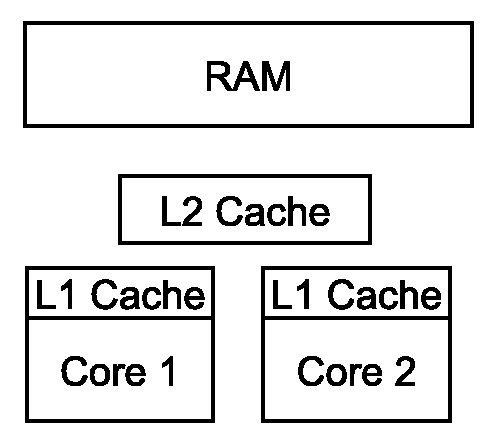
\includegraphics[scale=0.5]{Bilder/multicore.pdf}  
    	\textsf{\caption{Vereinfachte Ansicht auf die Cache-Struktur zwischen den Kernen und dem Arbeitsspeicher}}
		\label{fig:multicore}
	\end{center}
	 
\end{figure}

\subsection*{Vorteile}
\label{sec:Multicore_Vorteile}

Während bei der Datenverarbeitung auf einem Prozessorkern eine Parallelität über verschiedene Algorithmen wie zum Beispiel Round-Robin vorgetäuscht werden, ermöglicht die Einführung von Multicoreprozessoren inzwischen eine echte parallele Verarbeitung der Daten. So können auf beiden Kernen verschiedene Aufgaben gelöst werden, was einen bemerkbaren Zuwachs an Performanz für den Nutzer bringt. Im Datenbankbereich eröffnen Multicoreprozessoren neue Möglichkeiten der Optimierung. So kann ein Leistunsgewinn über den gemeinsamen Cache (Last Level Cache) oder die Verbesserung der Algorithmen erzielt werden.

\subsection*{Schwierigkeiten}
\label{sec:Multicore_Schwierigkeiten}
Die echte Parallelität bringt natürlich auch Probleme mit sich. Der Verwaltungsaufwand für die Koordinierung steigt. Im erwähnten Last Level Cache muss zum Beispiel sichergestellt werden, dass 
die Daten konsistenz sind, wenn zwei Threads auf verschiedenen Prozessoren auf den selben Daten operieren. 

Ein weiteres Problem ist, dass die Leistungsoptimierung durch die neue Prozessorarchitektur erst anschlägt, wenn die Programme dafür angepasst worden sind. Das bedeutet natürlich, dass erst einmal Entwicklungskosten entstehen. Hinzu kommt, dass auch das Betriebssystem mehrere Kerne unterstützen muss! Wenn das Betriebssystem nicht dazu in der Lage ist, kann auch eine optimierte Datenbankinstallation darauf nicht das Potential nutzen.

\section{Datenbank Operationen}
\label{sec:Operationen}
In den meisten Szenarien werden auf Datenbanken deutlich mehr Lese- als Schreiboperationen durchgeführt. Aufgrund dieser Tatsache werden wir in unserer Ausarbeitung den Augenmerk auf lesende Operationen legen. Weiterhin bieten diese Operationen mehr Potential zur Optimierung. Eine besonders wichtige Operation im Umfeld der relationen Datenbanken ist der Verbund (Join), einer der rechenintensivsten und teuersten Operation. Die Daten sind in fast allen Fällen über mehrere Tabellen verteilt, um den Normalformen zu genügen. Der Endnutzer betrachtet immer nur die aufbereiteten Enddaten, die wieder zusammengefügt werden.

In diesem Kontext hat sich der Hash-Join für Equal-Joins etabliert, da die Kosten mit steigender Tabellengröße nicht so schnell anwächst wie andere Algorithmen. 

Andere Operationen wie \texttt{INSERT}, \texttt{UPDATE} und \texttt{DELETE} werden in dieser Ausarbeitung nicht beachtet.
